\documentclass[a4paper,12pt]{report}
\usepackage[MeX]{polski}
\usepackage{amsfonts}
\usepackage{color}
\usepackage{graphicx}
\usepackage[utf8]{inputenc}
\usepackage{mathtools}
\usepackage{enumerate}
\usepackage{bbm}
\usepackage[hidelinks]{hyperref}
\usepackage{amsthm}
\usepackage{multicol}
\usepackage{cancel}
\usepackage{amsmath}
\usepackage{makeidx}
\title{}
\author{Mariusz Motyl}
\newtheoremstyle{break}
	{\topsep}{\topsep}
	{\itshape}{}
	{\bfseries}{}
	{\newline}{}
\newtheoremstyle{defi}
	{\topsep}{\topsep}
	{\normalfont}{}
	{\bfseries}{}
	{\newline}{}
\theoremstyle{break}
\newtheorem{twr}{Twierdzenie}
\theoremstyle{definition}
\theoremstyle{defi}
\newtheorem{defi}{Definicja}
\theoremstyle{break}
\newtheorem{lem}{Lemat}
\theoremstyle{defi}
\newtheorem{prz}{Przykład}
\newcommand{\Var}{\text{Var}}
\newcommand{\Perp}{{\perp \! \! \! \perp}}
\begin{document}
\chapter*{Lista 1}
\addcontentsline{toc}{chapter}{Lista 1}
\subsection*{Zadanie 1}
\addcontentsline{toc}{section}{Zadanie 1}
Wykazać, że jeśli $ X_1,X_2,\dots $ są zmiennymi losowymi o jednakowych wartościach oczekiwanych $ \mathbb E X_i=m $ dla $ i=1,\dots $ to
\begin{gather*}
\mathbb E \left(\frac{1}{N}\sum_{i=1}^{N}X_i\right)=m
\end{gather*}
niezależnie od tego czy $ N $ jest ustaloną liczbą naturalną, czy zmienną losową niezależną od $ X_1,X_2,\dots  $

Rozwiązanie:
\begin{enumerate}[a)]
\item 
\begin{align*}
&\mathbb E  \left(\frac{1}{N}\sum_{i=1}^{N}X_i\right)
=\\=&
\frac{1}{N} \mathbb E \left(\sum_{i=1}^{N}X_i\right)
=\\=&
\frac{1}{N}\sum_{i=1}^{N} \mathbb E \left(X_i\right)
=\\=&
\frac{1}{N}\sum_{i=1}^{N} m
=\\=&
\frac{N}{N}\cdot m=m
\end{align*}
\item 
\begin{align*}
&\mathbb E  \left(\frac{1}{N}\sum_{i=1}^{N}X_i\right)
=\\=&
\sum_{n=1}^{\infty }\mathbb E  \left(\frac{1}{N}\sum_{i=1}^{N}X_i|N=n\right)P\left(N=n\right)
=\\=&
\sum_{n=1}^{\infty }\mathbb E  \left(\frac{1}{n}\sum_{i=1}^{n}X_i\right)P\left(N=n\right)
=\\=&
\sum_{n=1}^{\infty }m\cdot P\left(N=n\right)=m
\end{align*}
\end{enumerate}


\subsection*{Zadanie 2}
\addcontentsline{toc}{section}{Zadanie 2}
Zmienna losowa $ X $ ma rozkład jednostajny na przedziale $ (0,1) $. Obliczyć wartość oczekiwaną zmiennej losowej $ Y=\min\left\{\frac{X}{1-X},\frac{1-X}{X}\right\} $.

Rozwiązanie:
\begin{itemize}
\item $ f_X(t)=\mathbbm1_{(0,1)}(t) $
\end{itemize}
\begin{gather*}
\frac{X}{1-X}=\frac{1-X}{X}\\
X^2=\left(1-X\right)^2\\
X^2-\left(1-X\right)^2=0\\
\left(2X-1\right)\cdot 1=0\\
X=\tfrac{1}{2}
\end{gather*}
\begin{align*}
\mathbb E Y=&\mathbb E \min\left\{\tfrac{X}{1-X},\tfrac{1-X}{X}\right\}
=\\=&
\int\limits_{0}^{1} \min\left\{\tfrac{x}{1-x},\tfrac{1-x}{x}\right\}f_X(x)\,dx
=\\=&
\int\limits_{0}^{\frac{1}{2}}\tfrac{x}{1-x}f_X(x)\,dx
+
\int\limits_{\frac{1}{2}}^{1}\tfrac{1-x}{x}f_X(x)\,dx
=\\=&
\int\limits_{0}^{\frac{1}{2}}\frac{x}{1-x}\,dx
+
\int\limits_{\frac{1}{2}}^{1}\frac{1-x}{x}\,dx
=\\=&
\int\limits_{0}^{\frac{1}{2}}\frac{1}{1-x}-1\,dx
+
\int\limits_{\frac{1}{2}}^{1}\frac{1}{x}-1\,dx
=\\=&
\ln \tfrac{1}{2}-\ln 1+\ln1-\ln\tfrac{1}{2}-1
=\\=&
2\ln2-1
\end{align*}


\subsection*{Zadanie 4}
\addcontentsline{toc}{section}{Zadanie 4}
Niech $ X_1,\dots,X_n$ będzie ciągiem zmiennych niezależnych zmiennych losowych o rozkładzie dwumianowym $ Ber(n_i,p) $, $ 1\le i\le n $. Wykazać, że zmienna losowa $ Y=X_1+\dots+X_n $ ma rozkład dwumianowy.

Rozwiązanie:
\begin{itemize}
\item $ \varphi _{Ber}(t)=\left(q+p^{it}\right)^n$
\end{itemize}

\begin{align*}
\varphi_{Y}=\varphi_{X_1+\dots+X_n}(t)\stackrel{\Perp}{=}&
\prod_{j=1}^{n}\varphi_{X_j}
=
\prod_{j=1}^{n}\left(q+p^{it}\right)^{n_j}
=
\left(q+p^{it}\right)^{\sum_{j=1}^{n}n_j}
\end{align*}
\begin{gather*}
Y\sim Ber\left(\sum_{j=1}^{n}n_j,p\right)
\end{gather*}


\newpage
\subsection*{Zadanie 5}
\addcontentsline{toc}{section}{Zadanie 5}
Niech $ X_1,\dots,X_n$ będzie ciągiem zmiennych niezależnych zmiennych losowych o rozkładzie Poissona $ P(\lambda_i) $, $ 1\le i\le n $. Wykazać, że zmienna losowa $ Y=X_1+\dots+X_n $ ma rozkład Poissona.

Rozwiązanie:
\begin{itemize}
\item $ \varphi_P(t)=e^{\lambda(e^{it}-1)}=\exp\bigl(\lambda(e^{it}-1)\bigr) $
\end{itemize}
\begin{gather*}
\varphi_{Y}=\varphi_{X_1+\dots+X_n}(t)\stackrel{\Perp}{=}
\prod_{j=1}^{n}\varphi_{X_j}
=
\prod_{j=1}^{n}\exp\bigl(\lambda_j(e^{it}-1)\bigr)
=
\exp\left(\sum_{j=1}^{n}\lambda_j(e^{it}-1)\right)
\end{gather*}
\begin{gather*}
Y\sim P\left(\sum_{j=1}^{n}\lambda_j\right)
\end{gather*}


\subsection*{Zadanie 6}
\addcontentsline{toc}{section}{Zadanie 6}
Niech $ X_1,\dots,X_n$ będzie ciągiem zmiennych niezależnych zmiennych losowych o rozkładzie Cauchy'ego $ C(\alpha_i,\lambda_i) $, $ \alpha_i\in \mathbb R ,\;\lambda_i>0,\;1\le i\le n $. Wykazać, że zmienna losowa $ Y=X_1+\dots+X_n $ ma rozkład Cauchy'ego.

Rozwiązanie:
\begin{itemize}
\item $ \varphi_X(t; \alpha_i,\lambda_i)
=
\mathbb E \left[e^{iXt} \right ]
=
e^{i\alpha_it - \lambda_i |t|} $
\end{itemize}
\begin{gather*}
\varphi_{Y}=\varphi_{X_1+\dots+X_n}(t)\stackrel{\Perp}{=}
\prod_{j=1}^{n}\varphi_{X_j}
=
\prod_{j=1}^{n}e^{i\alpha_jt - \lambda_j |t|}
=\\=
\exp \left({\sum_{j=1}^{n}i\alpha_jt - \lambda_j |t|}\right)
=
\exp \left({\sum_{j=1}^{n}i\alpha_jt - \sum_{j=1}^{n}\lambda_j |t|}\right)
\end{gather*}
\begin{gather*}
Y\sim C\left(\sum_{j=1}^{n}\alpha_j,\sum_{j=1}^{n}\lambda_j\right)
\end{gather*}


\newpage
\subsection*{Zadanie 7}
\addcontentsline{toc}{section}{Zadanie 7}
Niech $ X_1,\dots,X_n$ będzie ciągiem zmiennych niezależnych zmiennych losowych o rozkładzie wykładniczym z parametrem $ \lambda>0 $. Wyznaczyć rozkład zmiennej losowej $ Y=X_1+\dots+X_n $.

Rozwiązanie:
\begin{itemize}
\item $ \varphi_{Exp}(t)=\frac{\lambda}{\lambda-it} $
\item $ \varphi_{\Gamma}(t)=\left(\frac{1}{1-it\lambda}\right)^p$
\end{itemize}
\begin{gather*}
\varphi_{Y}=\varphi_{X_1+\dots+X_n}(t)\stackrel{\Perp}{=}
\prod_{j=1}^{n}\varphi_{X_j}
=
\prod_{j=1}^{n}\frac{\lambda}{\lambda-it}
=
\left(\frac{\lambda}{\lambda-it}\right)^n
=
\left(\frac{1}{1-\frac{it}{\lambda}}\right)^n
\end{gather*}
\begin{gather*}
Y\sim \Gamma\left(\tfrac{1}{\lambda},n\right)
\end{gather*}


\subsection*{Zadanie 8}
\addcontentsline{toc}{section}{Zadanie 8}
Niech zmienna losowa $ U $ ma rozkład jednostajny na przedziale $ (0,1) $ i niech $ F $ będzie dystrybuantą pewnego rozkładu. Wykazać, że zmienna losowa $ Y=F^{-1}(U) $ ma dystrybuantę $ F $.

Rozwiązanie:
\begin{align*}
F_Y(t)
=&
P\left(Y\le t\right)
=\\=&
P\left(F^{-1}(U)\le t\right)
=\\=&
P\bigl(U\le F(t)\bigr)
=\\=&
F\bigl(F(t)\bigr)=F(t)
\end{align*}
Do uzupełnienia formalizmów (trochę tego będzie).


\subsection*{Zadanie 9}
\addcontentsline{toc}{section}{Zadanie 9}
Zmienne losowe $ X $ i $ Y $ są niezależne o gęstościach:
\begin{align*}
&f_X(x)=\left \{
\begin{array}{cl}
	2x & \text{dla }x\in(0,1)   \\
	0  & \text{dla pozostałych}
\end{array}
\right .
&&x\in \mathbb R, \\
&f_Y(y)=\left \{
\begin{array}{cl}
	e^{-y} & \text{dla }y>0         \\
	  0    & \text{dla pozostałych}
\end{array}
\right .
&&y\in \mathbb R.
\end{align*}
Niech $ S=X+Y $. Obliczyć $ \mathbb E \left(S|X\le\frac{1}{2}\right) $.

Rozwiązanie:
\begin{align*}
\mathbb E \left(S|X\le\frac{1}{2}\right)=&
\frac{1}{P\left(X\le\frac{1}{2}\right)}\int\limits_{0}^{\frac{1}{2}}
\mathbb E \left(S|X=x\right)f_X(x)\,dx
=\\=&
\frac{1}{\int\limits_{0}^{\frac{1}{2}}2x\,dx}\int\limits_{0}^{\frac{1}{2}}
\mathbb E \left(X+Y|X=x\right)f_X(x)\,dx
=\\=&
4\int\limits_{0}^{\frac{1}{2}}
\mathbb E \left(x+Y|X=x\right)f_X(x)\,dx
=\\=&
4\int\limits_{0}^{\frac{1}{2}}
\mathbb E \left(x+Y|X=x\right)f_X(x)\,dx
=\\=&
4\int\limits_{0}^{\frac{1}{2}}
\mathbb E \left(x+Y\right)f_X(x)\,dx
=\\=&
4\int\limits_{0}^{\frac{1}{2}}
\bigl(\mathbb E \left(x\right) + \mathbb E \left(Y\right)\bigr)f_X(x)\,dx
=\\=&
4\int\limits_{0}^{\frac{1}{2}}
\bigl(x + \mathbb E \left(Y\right)\bigr)f_X(x)\,dx
=\\=&
4\int\limits_{0}^{\frac{1}{2}}
xf_X(x)\,dx + 
4\int\limits_{0}^{\frac{1}{2}}
\mathbb E \left(Y\right)f_X(x)\,dx
=\\=&
4\int\limits_{0}^{\frac{1}{2}}
x\cdot 2x\,dx + 
4\mathbb E \left(Y\right)\int\limits_{0}^{\frac{1}{2}}
2x\,dx
=\\=&
\frac{4}{12}+\frac{4}{4}\mathbb E \left(Y\right)
\end{align*}
$ \mathbb E \left(Y\right)=1 $
\begin{gather*}
\mathbb E \left(S|X\le\frac{1}{2}\right)=\frac{4}{3}
\end{gather*}


\subsection*{Zadanie 10}
\addcontentsline{toc}{section}{Zadanie 10}
Niech $ X $ i $ Y $ będą niezależnymi zmiennymi losowymi o rozkładach dwumianowych $ Ber(n,p) $ i $ Ber(m,p) $ odpowiednio. Wyznaczyć rozkład warunkowy zmiennej losowej $ X $ pod warunkiem $ X+Y=t $ oraz obliczyć $ \mathbb E \left(X|X+Y=t\right) $.

Rozwiązanie:
\begin{itemize}
\item 
\begin{gather*}
f_{X|Y}(x)=\frac{f_{X,Y}(x,y)}{\int\limits_{-\infty }^{\infty }f_{X,Y}(x,y)\,dy}
\end{gather*}
\item $ P\left(X=k\right)=\binom{n}{k}p^{k}(1-p)^{n-k} $
\end{itemize}
\begin{align*}
P\left(X+Y=t\right)=&
\sum_{k=0}^{t}P\left(X+Y=t|Y=k\right)P\left(Y=k\right)
\stackrel{\Perp}{=}\\=&
\sum_{k=0}^{t}P\left(X+k=t\right)P\left(Y=k\right)
=\\=&
\sum_{k=0}^{t}P\left(X=t-k\right)P\left(Y=k\right)
=\\=&
\sum_{k=0}^{t}
\binom{n}{t-k}p^{t-k}(1-p)^{n-t+k}
\binom{m}{k}p^{k}(1-p)^{m-k}
=\\=&
\sum_{k=0}^{t}
\binom{n}{t-k}\binom{m}{k}p^{t}(1-p)^{n+m-t}
=\\=&
p^{t}(1-p)^{n+m-t}\sum_{k=0}^{t}
\binom{n}{t-k}\binom{m}{k}
=\\=&
\binom{m+n}{t}p^{t}(1-p)^{n+m-t}
\end{align*}
Uzasadnienie ostatniego przejścia:
\begin{gather*}
\sum_{k=0}^{n+m}\binom{n+m}{k}x^t
=
\left(1+x\right)^{n+m}
=
\left(1+x\right)^{n}
\left(1+x\right)^{m}
=\\=
\Biggl(\sum_{k=0}^{n}\binom{n}{k}x^k\Biggr)
\Biggl(\sum_{j=0}^{m}\binom{m}{j}x^j\Biggr)
=\\=
\sum_{k=0}^{m+n}\Biggl(\sum_{j=0}^k \binom{m}{k-j}\binom{n}{j}\Biggr) x^k
\end{gather*}
\begin{align*}
P\left(X=k|X+Y=t\right)=&\frac{P\left(X=k,X+Y=t\right)}{P\left(X+Y=t\right)}
=\\=&
\frac{P\left(X=k\right) P\left(Y=t-k\right)}{P\left(X+Y=t\right)}
=\\=&
\frac{\binom{n}{k}p^{k}(1-p)^{n-k}
\binom{m}{t-k}p^{t-k}(1-p)^{m-t+k}}
{\binom{m+n}{t}p^{t}(1-p)^{n+m-t}}
=\\=&
\frac{\binom{n}{k}\binom{m}{t-k}p^{t}(1-p)^{n+m-t}}
{\binom{m+n}{t}p^{t}(1-p)^{n+m-t}}
=\\=&
\frac{\binom{n}{k}\binom{m}{t-k}}
{\binom{m+n}{t}}
\end{align*}
\begin{align*}
\mathbb E \left(X=k|X+Y=t\right)=&
\sum_{k=0}^{t}\frac{\binom{n}{k}\binom{m}{t-k}}
{\binom{m+n}{t}}k
\stackrel{wikipedia}{=}
\frac{nt}{m+n}
\end{align*}


\subsection*{Zadanie 11}
\addcontentsline{toc}{section}{Zadanie 11}
Niech $ N_1,N_2 $ będą niezależnymi zmiennymi losowymi o rozkładzie Poissona z parametrem $ \lambda_1=20$ i $ \lambda_2=30 $ odpowiednio. Obliczyć wariancję warunkową: $ \Var\left(N_1|N_1+N_2=50\right) $.

Rozwiązanie:
\begin{itemize}
\item $ \varphi_{Poiss}(t)=\exp \bigl(\lambda(e^{it}-1)\bigr) $
\item $ P\left(Poiss=t\right)=\frac{\lambda^t}{t!}e^{-\lambda} $
\end{itemize}
\begin{align*}
\varphi_{N_1+N_2}(t)
=&
\varphi_{N_1}(t)\varphi_{N_2}(t)
=\\=&
\exp \bigl(\lambda_1(e^{it}-1)\bigr)\exp \bigl(\lambda_2(e^{it}-1)\bigr)
=\\=&
\exp \bigl(\left(\lambda_1+\lambda_2\right)(e^{it}-1)\bigr)
\end{align*}
\begin{align*}
P \left(N_1=t|N_1+N_2=50\right)
=&
\frac{P\left(N_1=t,N_1+N_2=50\right)}{P\left(N_1+N_2=50\right)}
=\\=&
\frac{P\left(N_1=t,N_2=50-t\right)}{P\left(N_1+N_2=50\right)}
=\\=&
\frac{P\left(N_1=t\right) P\left(N_2=50-t\right)}{P\left(N_1+N_2=50\right)}
=\\=&
\frac{\frac{\lambda_1^t}{t!}e^{-\lambda_1}
\cdot
\frac{\lambda_2^{50-t}}{(50-t)!}e^{-\lambda_2}}{\frac{(\lambda_1+\lambda_2)^{50}}{50!}e^{-\lambda_1-\lambda_2}}
=\\=&
\frac{50!}{t!(50-t)!}\cdot \frac{20^t\cdot30^{50-t}}{(20+30)^{50}}
=\\=&
\binom{50}{t}\cdot \left(\frac{2}{5}\right)^t\cdot \left(\frac{3}{5}\right)^{50-t}
\end{align*}
\begin{gather*}
\left(N_1=t|N_1+N_2=50\right)\sim Ber(50,\tfrac{2}{5})\\
\Var\left(N_1=t|N_1+N_2=50\right)=
50\cdot\frac{2}{5}\cdot\frac{3}{5}=12
\end{gather*}


\subsection*{Zadanie 12}
\addcontentsline{toc}{section}{Zadanie 12}
Niech $ X_1,\dots,X_n$ będą niezależnymi zmiennymi losowymi o rozkładzie Poissona z parametrem $ \lambda>0 $. Znaleźć rozkład warunkowy zmiennej losowej $ X_1 $ pod warunkiem $ S_n $, gdzie $ S_n=\sum_{i=1}^{n}X_i $

Rozwiązanie:
\begin{itemize}
\item $ X_i\sim Poiss(\lambda) $
\item $ S_n\sim Poiss(n\lambda) $
\end{itemize}
\begin{align*}
P\left(X_1=t|S_n=k\right)\stackrel{\Perp}{=}&
\frac{P\left(X_1=t,S_n=k\right)}{P\left(S_n=k\right)}
=\\=&
\frac{P\left(X_1=t,X_2+\dots+X_n=k-t\right)}{P\left(S_n=k\right)}
=\\=&
\frac{P\left(X_1=t\right) P\left(X_2+\dots+X_n=k-t\right)}{P\left(S_n=k\right)}
=\\=&
\frac{\lambda^t}{t!}e^{-\lambda}
\cdot 
\frac{\bigl((n-1)\lambda\bigr)^{k-t}}{(k-t)!}e^{-(n-1)\lambda}
\cdot 
\frac{k!}{(n\lambda)^k}e^{n\lambda}
=\\=&
\frac{\lambda^t}{t!}
\cdot 
\frac{\bigl((n-1)\lambda\bigr)^{k-t}}{(k-t)!}
\cdot 
\frac{k!}{(n\lambda)^k}
=\\=&
\frac{(n-1)^{k-t}}{n^k}\cdot \frac{k!}{t!(k-t)!}
=\\=&
\left(\frac{n-1}{n}\right)^{k-t}\left(\frac{1}{n}\right)^t\binom{k}{t}
\end{align*}
\begin{gather*}
\left(X_1=t|S_n=k\right)\sim Ber(k,\tfrac{1}{n})
\end{gather*}
\chapter*{Lista 2}
\addcontentsline{toc}{chapter}{Lista 2}


\subsection*{Zadanie 13}
\addcontentsline{toc}{section}{Zadanie 13}
Niech $ N,X_1,X_2,\dots$ będzie ciągiem niezależnych zmiennych losowych. Zmienna losowa $ N $ ma rozkład Poissona z parametrem $ \lambda $, a zmienne losowe $ X_i $, dla $ i=1,2,\dots$ mają rozkład dwupunktowy tj.
\begin{gather*}
P\left\{X_i=1\right\}=\frac{2}{3},\qquad P\left\{X_i=2\right\}=\frac{1}{3}
\end{gather*}
Niech $ S_N=\sum_{i=1}^{N}X_i $. Obliczyć $ \mathbb E \left(N|S_N=3\right) $.

Rozwiązanie:
\begin{align*}
\mathbb E \left(N|S_N=3\right)=&
\sum_{k=0}^{\infty }k\cdot P\left(N=k|S_N=3\right)
=\\=&
2\cdot P\left(N=2|S_N=3\right)+3\cdot P\left(N=3|S_N=3\right)
=\\=&
2\cdot \frac{P\left(N=2,S_2=3\right)}{P\left(S_N=3\right)}
+
3\cdot \frac{P\left(N=3,S_3=3\right)}{P\left(S_N=3\right)}
=\\=&
2\cdot \frac{P\left(N=2\right) P\left(S_2=3\right)}{P\left(S_N=3\right)}
+
3\cdot \frac{P\left(N=3\right) P\left(S_3=3\right)}{P\left(S_N=3\right)}
=\\=&
2\cdot \frac{\lambda^2}{2!}e^{-\lambda}\cdot \frac{ P\left(S_2=3\right)}{P\left(S_N=3\right)}
+
3\cdot \frac{\lambda^3}{3!}e^{-\lambda}\cdot\frac{P\left(S_3=3\right)}{P\left(S_N=3\right)}
=\\=&
\frac{1}{P\left(S_N=3\right)}\cdot\left( \lambda^2e^{-\lambda}\cdot  P\left(S_2=3\right)
+
\frac{\lambda^3}{2}e^{-\lambda}\cdot P\left(S_3=3\right)\right)
\end{align*}
\begin{align*}
P\left(S_2=3\right)=&
P\left(X_1=1\right)P\left(X_2=2\right)
+
P\left(X_1=2\right)P\left(X_2=1\right)
=\\=&
\frac{2}{3}\cdot \frac{1}{3}
+
\frac{1}{3}\cdot \frac{2}{3}=\frac{4}{9}
\end{align*}
\begin{align*}
P\left(S_3=3\right)=&
P\left(X_1=1\right)P\left(X_2=1\right)P\left(X_3=1\right)
=\\=&
\left(\frac{1}{3}\right)^3=\frac{1}{27}
\end{align*}
\begin{align*}
P\left(S_N=3\right)=&
\sum_{n=0}^{\infty }P\left(S_N=3|N=n\right)P\left(N=n\right)
=\\=&
\sum_{n=0}^{\infty }P\left(S_n=3\right)P\left(N=n\right)
=\\=&
P\left(S_2=3\right)P\left(N=2\right)+P\left(S_3=3\right)P\left(N=3\right)
=\\=&
\frac{4}{9}\cdot \frac{\lambda^2}{2!}e^{-\lambda}
+
\frac{1}{27}\cdot \frac{\lambda^3}{3!}e^{-\lambda}
=\\=&
\frac{1}{162} \lambda ^3 e^{-\lambda }+\frac{2}{9} \lambda ^2 e^{-\lambda }
\end{align*}
\begin{align*}
\mathbb E \left(N|S_N=3\right)=&
\frac{1}{P\left(S_N=3\right)}\cdot\left( \lambda^2e^{-\lambda}\cdot  P\left(S_2=3\right)
+
\frac{\lambda^3}{2}e^{-\lambda}\cdot P\left(S_3=3\right)\right)
=\\=&
\frac{1}{\frac{1}{162} \lambda ^3 e^{-\lambda }+\frac{2}{9} \lambda ^2 e^{-\lambda }}\cdot
\left( \lambda^2e^{-\lambda}\cdot  \frac{4}{9}
+
\frac{\lambda^3}{2}e^{-\lambda}\cdot \frac{1}{27}\right)
=\\=&
\frac{\frac{1}{54} \lambda ^2 (\lambda +24) e^{-\lambda }}{\frac{1}{162} \lambda ^2 (\lambda +36) e^{-\lambda }}
=\\=&
\frac{3 (\lambda +24)}{\lambda +36}
\end{align*}


\subsection*{Zadanie 14}
\addcontentsline{toc}{section}{Zadanie 14}
Zmienna losowa $ X $ ma rozkład Poissona z parametrem $ \lambda $. Rozkład warunkowy zmiennej losowej $ Y $ przy warunku $ X=k $ jest rozkładem dwumianowym z parametrami $ (k,p) $. Wykazać, że zmienna losowa $ Y $ ma Rozkład Poissona z parametrem $ \lambda p $. Następnie wykazać niezależność zmiennych losowych $ Y $ i $ X-Y $ oraz wyznaczyć rozkład warunkowy $ X $ przy warunku $ Y=y $.

Rozwiązanie:
\begin{itemize}
\item $ X\sim Poisson(\lambda) $
\item $ (Y|X=k)\sim Ber(k,p) $
\end{itemize}
\begin{gather*}
P\left(Y=t|X=n\right)=
\frac{P\left(Y=t,X=n\right)}{P\left(X=n\right)}=
\binom{k}{t}p^t(1-p)^{k-t}
\end{gather*}
\begin{align*}
\frac{P\left(Y=t,X=k\right)}{P\left(X=k\right)}=&
\binom{k}{t}p^t(1-p)^{k-t}\\
P\left(Y=t,X=k\right)=&
\binom{k}{t}p^t(1-p)^{k-t}P\left(X=k\right)\\
P\left(Y=t,X=k\right)=&
\frac{k!}{t!(k-t)!}p^t(1-p)^{k-t}\frac{\lambda^k}{k!}e^{-\lambda}\\
P\left(Y=t,X=k\right)=&
\frac{e^{-\lambda } \lambda ^k p^t (1-p)^{k-t}}{t! (k-t)!}
\end{align*}
\begin{gather*}
P\left(Y=t\right)=\sum_{k=0}^{\infty }P\left(Y=t,X=k\right)
\end{gather*}\begin{align*}
P\left(Y=t\right)=&\sum_{k=0}^{\infty }P\left(Y=t,X=k\right)
=\\=&
\sum_{k=t}^{\infty }\frac{e^{-\lambda } \lambda ^k p^t (1-p)^{k-t}}{t! (k-t)!}
=\\=&
\frac{ p^t\lambda^t}{t!}e^{-\lambda}\cdot
\sum_{k=t}^{\infty }\frac{ \lambda ^{k-t} (1-p)^{k-t}}{ (k-t)!}
=\\=&
\frac{ p^t\lambda^t}{t!}e^{-\lambda}\cdot
\sum_{k=0}^{\infty }\frac{ \bigl(\lambda (1-p)\bigr)^{k}}{k!}
=\\=&
\frac{ p^t\lambda^t}{t!}e^{-\lambda}\cdot
e^{\lambda (1-p)}
=\\=&
\frac{ p^t\lambda^t}{t!}e^{-\lambda}\cdot
e^{\lambda (1-p)}
=\\=&
\frac{ (p\lambda)^t}{t!}e^{-p\lambda}
\end{align*}
\begin{align*}
P\left(X-Y=n\right)=&
\sum_{k=n}^{\infty }P\left(X-Y=n|X=k\right)P\left(X=k\right)
=\\=&
\sum_{k=n}^{\infty }P\left(Y=k-n|X=k\right)P\left(X=k\right)
=\\=&
\sum_{k=n}^{\infty }P\left(Y=k-n,X=k\right)
=\\=&
\sum_{k=n}^{\infty }\frac{e^{-\lambda } \lambda ^k p^{k-n} (1-p)^{n}}{(k-n)! n!}
=\\=&
\frac{e^{-\lambda } (1-p)^{n}}{n!}\cdot
\sum_{k=n}^{\infty }\frac{\lambda ^k p^{k-n} }{(k-n)! }
=\\=&
\frac{e^{-\lambda } (1-p)^{n}}{n!}\cdot \lambda^n\cdot
\sum_{k=0}^{\infty }\frac{(\lambda p)^{k} }{k!}
=\\=&
\frac{e^{-\lambda } (1-p)^{n}}{n!}\cdot \lambda^n
e^{\lambda p}
=\\=&
\frac{e^{-\lambda } \lambda ^n (1-p)^n e^{p\lambda}}{n!}
\end{align*}
\begin{align*}
P\left(X-Y=n\right)P\left(Y=t\right)=&
\frac{e^{-\lambda } \lambda ^n (1-p)^n e^{p\lambda}}{n!}
\cdot \frac{ (p\lambda)^t}{t!}e^{-p\lambda}
=\\=&
\frac{\lambda ^n (1-p)^n e^{-\lambda} (\lambda  p)^t}{n! t!}
\end{align*}
\begin{align*}
P\left(X-Y=n,Y=t\right)=&
P\left(X=n+t,Y=t\right)
=\\=&
\frac{e^{-\lambda } p^t (1-p)^n \lambda ^{t+n}}{t! n!}
\end{align*}
\begin{gather*}
P\left(X-Y=n,Y=t\right)=P\left(X-Y=n\right)P\left(Y=t\right)
\end{gather*}
\begin{align*}
P\left(X=k|Y=t\right)=&
\frac{P\left(X=k,Y=t\right)}{P\left(Y=t\right)}
=\\=&
\frac{e^{-\lambda } \lambda ^k p^t (1-p)^{k-t}}{t! (k-t)!}
\cdot \frac{t!}{ (p\lambda)^t}e^{p\lambda}
=\\=&
\frac{\lambda ^{k-t} e^{\lambda  (p-1)} (1-p)^{k-t} }{(k-t)!}
\end{align*}


\subsection*{Zadanie 15}
\addcontentsline{toc}{section}{Zadanie 15}
Niech będzie dane $ \sigma $-ciało $ \mathcal B $ generowane przez skończone lub przeliczalne nieskończone rozbicie $ \left\{A_i\right\}_{i\in I} $ zbioru $ \Omega $. Wykazać
\begin{gather*}
P\left(B|\mathcal B\right)=\sum_{i\in I,P\left(A_i\right)>0}P\left(B|A_i\right)I_{A_i},\qquad B\in \mathcal F 
\end{gather*}
oraz dla całkowalnej zmiennej losowej $ X $ $ \left(\mathbb E \left|X\right|<\infty \right) $
\begin{gather*}
\mathbb E \left(X|\mathcal B\right)=\sum_{i\in I,P\left(A_i\right)>0}\frac{1}{P\left(A_i\right)}\int\limits_{A_i}X(\omega)\,dP(\omega)I_{A_i}
\end{gather*}
Rozwiązanie:
\begin{align*}
&\mathbb E \left(\mathbbm1_{B}|\mathcal B\right)
\stackrel{df}{=}\\=&
\sum_{i\in I}\mathbb E \left(\mathbbm1_{B}|A_i\right)\cdot\mathbbm1_{A_i}
=\\=&
\sum_{i\in I,P\left(A_i\right)>0}
\frac{1}{P\left(A_i\right)}\int\limits_{A_i}\mathbbm1_{B}\,dP\cdot\mathbbm1_{A_i}
=\\=&
\sum_{i\in I,P\left(A_i\right)>0}
\frac{P\left(A_i\cap B\right)}{P\left(A_i\right)}
=\\=&
\sum_{i\in I,P\left(A_i\right)>0}
P\left(B|A_i\right)\cdot\mathbbm1_{A_i}
\end{align*}
Komentarz chyba wymaga, żeby podkreślić, iż zmienna losowa $ Y(\omega)=\mathbbm1_{B}(\omega) $ dla $ B\in\mathcal B $ jest całkowalna, a jest, bo niezależnie od $ B $ mamy $ \mathbb E \left(\mathbbm1_{B}\right)=P\left(B\right)\le1<\infty  $, czyli wszystko gra.\\
Druga część analogicznie, ale wiemy, że $ E\left(|X|\right)<\infty  $
\begin{align*}
&\mathbb E \left(X|\mathcal B\right)
\stackrel{df}{=}\\=&
\sum_{i\in I}\mathbb E \left(X|A_i\right)\cdot\mathbbm1_{A_i}
=\\=&
\sum_{i\in I,P\left(A_i\right)>0}
\frac{1}{P\left(A_i\right)}\int\limits_{A_i}X(\omega)\,dP\cdot\mathbbm1_{A_i}
\end{align*}

\subsection*{Zadanie 16 - poprawione}
\addcontentsline{toc}{section}{Zadanie 16 - poprawione}
Niech $ \Omega=[0,1] $, a $ P $ będzie miarą Lebegue'a na zbiorach borelowskich $ \Omega $. Niech $ \mathcal B $ będzie $ \sigma $-algebrą generowaną przez rodzinę zbiorów\\ $ \left\{\left[0,\frac{1}{3}\right) ,\left\{\frac{1}{3}\right\},\left(\frac{1}{3},\frac{1}{2}\right]\right\} $. Wyznaczyć dwie różne wersje $ \mathbb E \left(X|\mathcal B\right) $, jeśli:
\begin{enumerate}[(a)]
\item $ X(\omega)=\omega $
\item $ X(\omega)=\sin\pi\omega $
\item $ X(\omega)=\omega^2 $
\item $ X(\omega)=1-\omega $
\item 
\begin{gather*}
X(\omega)=\left \{
\begin{array}{ll}
	1, & \omega\in\left[0,\frac{1}{3}\right] \\
	2, & \omega\in\left (\frac{1}{3},1\right ]
\end{array}
\right .
\qquad\omega\in\Omega
\end{gather*}
\end{enumerate}

Rozwiązanie:
\begin{gather*}
\mathbb{E}(X|\mathcal F_0)(\omega)=\sum_{j=1}\mathbb{E}(X|A_j)\mathbbm{1}_{A_j}(\omega)
\end{gather*}
\begin{enumerate}[(a)]
\item 
\begin{align*}
&\mathbb E \left(X(\omega)|\mathcal B\right)
=\\=&
\mathbb E \left(\omega|\mathcal B\right)
=\\=&
\mathbb E \left(\omega|\left[0,\tfrac{1}{3}\right)\right)
\mathbbm1_{\left[0,\frac{1}{3}\right)}(\omega)
+
\mathbb E \left(\omega|\left\{\tfrac{1}{3}\right\}\right)
\mathbbm1_{\left\{\frac{1}{3}\right\}}(\omega)
+\\+&
\mathbb E \left(\omega|\left(\tfrac{1}{3},\tfrac{1}{2}\right]\right)
\mathbbm1_{\left(\frac{1}{3},\frac{1}{2}\right]}(\omega)
+
\mathbb E \left(\omega|\left(\tfrac{1}{2},1\right]\right)
\mathbbm1_{\left(\frac{1}{2},1\right]}(\omega)
=\\=&
\int\limits_{0}^{\frac{1}{3}}\omega\,d\lambda(\omega)
\mathbbm1_{\left[0,\frac{1}{3}\right)}(\omega)
+
\mathbbm1_{\left\{\frac{1}{3}\right\}}(\omega)
+
\int\limits_{\frac{1}{3}}^{\frac{1}{2}}\omega\,d\lambda(\omega)
\mathbbm1_{\left(\frac{1}{3},\frac{1}{2}\right]}(\omega)
+
\int\limits_{\frac{1}{2}}^{1}\omega\,d\lambda(\omega)
\mathbbm1_{\left(\frac{1}{2},1\right]}(\omega)
=\\=&
\frac{1}{18}
\mathbbm1_{\left[0,\frac{1}{3}\right)}(\omega)
+
\mathbbm1_{\left\{\frac{1}{3}\right\}}(\omega)
+
\frac{5}{72}
\mathbbm1_{\left(\frac{1}{3},\frac{1}{2}\right]}(\omega)
+
\frac{3}{8}
\mathbbm1_{\left(\frac{1}{2},1\right]}(\omega)
\end{align*}
Drugie
\begin{align*}
&\mathbb E \left(X(\omega)|\mathcal B\right)
=\\=&
\mathbb E \left(\omega|\mathcal B\right)
=\\=&
\mathbb E \left(\omega|\left[0,\tfrac{1}{3}\right]\right)
\mathbbm1_{\left[0,\frac{1}{3}\right]}(\omega)
+
\mathbb E \left(\omega|\left(\tfrac{1}{3},\tfrac{1}{2}\right]\right)
\mathbbm1_{\left(\frac{1}{2},1\right]}(\omega)
=\\=&
\int\limits_{0}^{\frac{1}{3}}\omega\,d\lambda(\omega)
\mathbbm1_{\left[0,\frac{1}{3}\right]}(\omega)
+
\int\limits_{\frac{1}{3}}^{\frac{1}{2}}\omega\,d\lambda(\omega)
\mathbbm1_{\left(\frac{1}{3},\frac{1}{2}\right]}(\omega)
+
\int\limits_{\frac{1}{2}}^{1}\omega\,d\lambda(\omega)
\mathbbm1_{\left(\frac{1}{2},1\right]}(\omega)
=\\=&
\frac{1}{18}
\mathbbm1_{\left[0,\frac{1}{3}\right]}(\omega)
+
\frac{5}{72}
\mathbbm1_{\left(\frac{1}{3},\frac{1}{2}\right]}(\omega)
+
\frac{3}{8}
\mathbbm1_{\left(\frac{1}{2},1\right]}(\omega)
\end{align*}
\end{enumerate}


\subsection*{Zadanie 17}
\addcontentsline{toc}{section}{Zadanie 17}
Niech $ \Omega=[0,1] $, a $ P $ będzie miarą Lebegue'a na zbiorach borelowskich $ \Omega $. Niech $ \mathcal B $ będzie $ \sigma $-algebrą generowaną przez rodzinę zbiorów $ \left\{\left[0,\frac{1}{4}\right),\left[\frac{1}{4},\frac{3}{4}\right),\left[\frac{3}{4},1\right]\right\} $. Wyznaczyć $ P\left(\cdot|\mathcal B\right) $ oraz $ \mathbb E \left(X|\mathcal B\right) $, gdzie $ X(\omega)=\omega^2,\omega\in\Omega $.

Rozwiązanie:
\begin{itemize}
\item Odwołując się do zadania 15
\begin{gather*}
P\left(B|\mathcal B\right)=\sum_{i\in I,P\left(A_i\right)>0}P\left(B|A_i\right)I_{A_i},\qquad B\in \mathcal F 
\end{gather*}
\item Podobnie
\begin{gather*}
\mathbb E \left(X|\mathcal B\right)=\sum_{i\in I,P\left(A_i\right)>0}\frac{1}{P\left(A_i\right)}\int\limits_{A_i}X(\omega)\,dP(\omega)I_{A_i}
\end{gather*}
\end{itemize}
Na start
\begin{align*}
&P\left(\left[0,\tfrac{1}{4}\right)\right)=\frac{1}{4}\\
&P\left(\left[\tfrac{1}{4},\tfrac{3}{4}\right)\right)=\frac{1}{2}\\
&P\left(\left[\tfrac{3}{4},1\right]\right)=\frac{1}{4}
\end{align*}
\begin{align*}
&P\left(Y|\mathcal B\right)
=\\=&
P\left(Y|\left[0,\tfrac{1}{4}\right)\right)
\mathbbm1_{\left[0,\tfrac{1}{4}\right)}+
P\left(Y|\left[\tfrac{1}{4},\tfrac{3}{4}\right)\right)
\mathbbm1_{\left[\tfrac{1}{4},\tfrac{3}{4}\right)}+
P\left(Y|\left[\tfrac{3}{4},1\right]\right)
\mathbbm1_{\left[\tfrac{3}{4},1\right]}
=\\=&
\frac{P\left(Y\cap \left[0,\tfrac{1}{4}\right)\right)}{P\left(\left[0,\tfrac{1}{4}\right)\right)}
\mathbbm1_{\left[0,\frac{1}{4}\right)}+
\frac{P\left(Y\cap \left[\tfrac{1}{4},\tfrac{3}{4}\right)\right)}{P\left(\left[\tfrac{1}{4},\tfrac{3}{4}\right)\right)}
\mathbbm1_{\left[\frac{1}{4},\frac{3}{4}\right)}+
\frac{P\left(Y\cap \left[\tfrac{3}{4},1\right]\right)}{P\left(\left[\tfrac{3}{4},1\right]\right)}
\mathbbm1_{\left[\frac{3}{4},1\right]}
=\\=&
4\cdot P\left(Y\cap \left[0,\tfrac{1}{4}\right)\right)
\mathbbm1_{\left[0,\frac{1}{4}\right)}+
2\cdot P\left(Y\cap \left[\frac{1}{4},\frac{3}{4}\right)\right)
\mathbbm1_{\left[\frac{1}{4},\frac{3}{4}\right)}+
4\cdot P\left(Y\cap \left[\frac{3}{4},1\right]\right)
\mathbbm1_{\left[\frac{3}{4},1\right]}
\end{align*}
Wartość oczekiwana
\begin{align*}
&\mathbb E \left(X|\mathcal B\right)
=\\=&
\mathbbm1_{\left[0,\frac{1}{4}\right)}
\mathbb E \left(X|\left[0,\tfrac{1}{4}\right)\right)+
\mathbbm1_{\left[\frac{1}{4},\frac{3}{4}\right)}
\mathbb E \left(X|\left[\tfrac{1}{4},\tfrac{3}{4}\right)\right)+
\mathbbm1_{\left[\frac{3}{4},1\right]}
\mathbb E \left(X|\left[\tfrac{3}{4},1\right]\right)
=\\=&
4\cdot\mathbbm1_{\left[0,\frac{1}{4}\right)}
\int\limits_{0}^{\frac{1}{4}}\omega^2\,dP+
2\cdot\mathbbm1_{\left[\frac{1}{4},\frac{3}{4}\right)}
\int\limits_{\frac{1}{4}}^{\frac{3}{4}}\omega^2\,dP+
4\cdot\mathbbm1_{\left[\frac{3}{4},1\right]}
\int\limits_{\frac{3}{4}}^1\omega^2\,dP
=\\=&
\frac{1}{48}\mathbbm1_{\left[0,\frac{1}{4}\right)}+
\frac{13}{48}\mathbbm1_{\left[\frac{1}{4},\frac{3}{4}\right)}+
\frac{37}{48}\mathbbm1_{\left[\frac{3}{4},1\right]}
\end{align*}


\subsection*{Zadanie 20}
\addcontentsline{toc}{section}{Zadanie 20}
Niech $ X $ będzie nieujemną zmienną losową i niech $ \mathcal B\subset \mathcal F  $ będzie $ \sigma $-algebrą. Wykazać, że $ \mathbb E \left(X|\mathcal B\right)<\infty  $ ($ P $ - p.w.) wtedy i tylko wtedy, gdy miara $ Q $ określona wzorem
\begin{gather*}
Q(A)=\int\limits_{A}X(\omega)\,dP(\omega),\qquad
A\in B
\end{gather*}
jest $ \sigma $-skończona.

Rozwiązanie:
\begin{itemize}
\item Miara jest $ \sigma $-skończona, gdy przestrzeń, w której występuje może być przedstawiona jako suma przeliczalnie wielu zbiorów miary skończonej.
\end{itemize}
Gdy $ \left\{A_i\right\} \subset\mathcal B $ jest rozbiciem $ \Omega $
\begin{gather*}
\mathbb E \left(X|\mathcal B\right)=\sum_i \mathbb E \left(X|A_i\right)\mathbbm1_{A_i}<\infty 
\end{gather*}
Czyli
\begin{align*}
&\forall_i \mathbb E \left(X|A_i\right)<\infty \\
&\forall_i \frac{1}{P\left(A_i\right)}\int\limits_{A_i}X(\omega)\,P(\omega)<\infty \\
&\forall_i \int\limits_{A_i}X(\omega)\,P(\omega)<\infty
\end{align*}
$ Q(A) $ jest $ \sigma $-skończona.

"$ \Leftarrow $" Gdy $ Q(A) $ jest $ \sigma $-skończona to dla $ A_i $ takich, że $ \bigcup_i A_i=\Omega $ oraz $ A_i\cap A_j=\emptyset $ dla $ i\neq j $
\begin{align*}
&Q(A_i)<\infty
\end{align*}
Dla $ A_i $ takich, że $ P(A_i)>0 $
\begin{gather*}
\frac{Q(A_i)}{P(A_i)}<\infty 
\end{gather*}
Pamiętając, że
\begin{gather*}
\mathbb E \left(X|\mathcal B\right)=
\sum_{i\in I,P\left(A_i\right)>0}\frac{1}{P\left(A_i\right)}\int\limits_{A_i}X(\omega)\,dP(\omega)I_{A_i}
=\\=
\sum_{i\in I,P\left(A_i\right)>0}\frac{Q(A_i)}{P\left(A_i\right)}I_{A_i}<\infty 
\end{gather*}
Ostatnia nierówność jest oczywista ze względu na funkcję charakterystyczną.


\subsection*{Zadanie 22}
\addcontentsline{toc}{section}{Zadanie 22}
Niech $ X,Y\in L^1\left(\Omega,\mathcal F, P\right) $ będą niezależnymi zmiennymi losowymi o takim samym rozkładzie. Wykazać, że
\begin{gather*}
\mathbb E \left(X|X+Y\right)=\mathbb E \left(Y|X+Y\right)=\frac{X+Y}{2},\qquad P\,\text{prawie wszędzie}
\end{gather*}

Rozwiązanie:
\begin{itemize}
\item 
\begin{gather*}
\mathbb E \left(X|X\right)
=
X
\end{gather*}
\end{itemize}
\begin{align*}
&\mathbb E \left(X|X+Y\right)
+
\mathbb E \left(Y|X+Y\right)
=
\mathbb E \left(X+Y|X+Y\right)
=
X+Y\\
&\mathbb E \left(X|X+Y\right)
=
\mathbb E \left(Y|X+Y\right)=\frac{X+Y}{2}
\end{align*}


\subsection*{Zadanie 24}
\addcontentsline{toc}{section}{Zadanie 24}
Zmienne losowe $ X $ i $ Y $ są niezależne o skończonej wariancji. Wykazać, że
\begin{gather*}
\Var\left(XY\right) = \mathbb E \bigl(\Var\left(XY|X\right)\bigr)+\Var\bigl(\mathbb E \left(XY|X\right)\bigr)
\end{gather*}

Rozwiązanie:
\begin{align*}
\Var\left(XY\right)=&\mathbb E \left(XY\right)^2-\bigl(\mathbb E \left(XY\right)\bigr)^2
\end{align*}
\begin{align*}
&\mathbb E \bigl(\Var\left(XY|X\right)\bigr)+\Var\bigl(\mathbb E \left(XY|X\right)\bigr)
=\\=&
\mathbb E \left(\mathbb E \left((XY)^2|X\right)-\bigl(\mathbb E \left((XY)^2|X\right)\bigr)\right)
+
\mathbb E \bigl(\mathbb E \left((XY)^2|X\right)\bigr)-\Bigl(\mathbb E \bigl(\mathbb E \left(XY|X\right)\bigr)\Bigr)^2
=\\=&
\mathbb E (XY)^2-\cancel{\mathbb E \bigl(\mathbb E \left((XY)^2|X\right)\bigr)}
+
\cancel{\mathbb E \bigl(\mathbb E \left((XY)^2|X\right)\bigr)}-\Bigl(\mathbb E \bigl(\mathbb E \left(XY|X\right)\bigr)\Bigr)^2
=\\=&
\mathbb E (XY)^2-\bigl(\mathbb E \left(XY\right)\bigr)^2
=\\=&
\Var\left(XY\right)
\end{align*}
\chapter*{Lista 3}
\addcontentsline{toc}{chapter}{Lista 3}


\subsection*{Zadanie 25}
\addcontentsline{toc}{section}{Zadanie 25}
Wykazać, że zmienna losowa $ X $ jest niezależna od $ \sigma $-algebry $ \mathcal B $ wtedy i tylko wtedy, gdy dla dowolnej funkcji borelowskiej ograniczonej $ \varphi $ takiej, że $ \mathbb E \left|\varphi(X)\right|<\infty  $ spełniony jest warunek
\begin{gather*}
\mathbb E \left(\varphi(X)|\mathcal B\right)=\mathbb E \varphi(X)
\end{gather*}

Rozwiązanie:
\begin{itemize}
\item $ \mathcal B=\sigma\left(A_1,A_2,\dots\right) $
\end{itemize}
"$ \Rightarrow $"
\begin{align*}
&\mathbb E \left(\varphi(X)|\mathcal B\right)
=\\=&
\sum_{i\in \mathbb N ,P\left(A_i\right)>0}
\mathbb E \left(\varphi(X)|\mathcal A_i\right)I_{A_i}
\stackrel{\Perp}{=}\\=&
\sum_{i\in \mathbb N ,P\left(A_i\right)>0}
\mathbb E \varphi(X)I_{A_i}
=\\=&
E\varphi(X)
\end{align*}
"$ \Leftarrow $" Dowód przez sprzeczność
\begin{align*}
\exists_{i\in \mathbb N }\mathbb E \left(\varphi(X)|\mathcal A_i\right)&\neq\mathbb E \left(\varphi(X)\right)\\
\sum_{i\in \mathbb N ,P\left(A_i\right)>0}
\mathbb E \left(\varphi(X)|\mathcal A_i\right)I_{A_i}&\neq
\sum_{i\in \mathbb N ,P\left(A_i\right)>0}
\mathbb E \varphi(X)I_{A_i}\\
\mathbb E \left(\varphi(X)|\mathcal B\right)&\neq
\mathbb E \varphi(X)
\end{align*}
czyli, $ \varphi(X) $ i $ A_i $ są zależne dla ustalonego $ i $, a tym samym $ \varphi(X) $ i $ \mathcal B $ są zależne. Czyli z prawa kontrapozycji zachodzi implikacja przeciwna.


\subsection*{Zadanie 31}
\addcontentsline{toc}{section}{Zadanie 31}
Niech dwuwymiarowy wektor losowy $ (X,Y) $ ma gęstość
\begin{gather*}
f(x,y)=\left \{
\begin{array}{lll}
	\frac{1}{\pi} & \text{dla} & x^2+y^2<1   \\
	0             & \text{dla} & x^2+y^2\ge1
\end{array}
\right .
(x,y)\in \mathbb R ^2
\end{gather*}
Wyznaczyć $ F_{X|Y} $ oraz obliczyć Cov$ (X,Y) $

Rozwiązanie:
\begin{align*}
&f_{X|Y}=\frac{f(x,y)}{\int\limits_{\mathbb R }f(x,y)\,dx}
=\\=&
\frac{1}{\pi}\mathbbm1_{\left\{x^2+y^2<1\right\}}(x,y)
\left(\int\limits_{-\sqrt{1-y^2}}^{\sqrt{1-y^2}}\frac{1}{\pi}\,dx\right)^{-1}
=\\=&
\frac{1}{\pi}\mathbbm1_{\left\{x^2+y^2<1\right\}}(x,y)\cdot
\frac{\pi}{2\sqrt{1-y^2}}
=\\=&
\frac{1}{2\sqrt{1-y^2}}\mathbbm1_{\left\{x^2+y^2<1\right\}}(x,y)
\end{align*}
\begin{align*}
\mathbb E Y=
\int\limits_{-1}^{1}\frac{y}{\pi}\cdot\frac{1}{2\sqrt{1-y^2}}\,dy=0
\end{align*}
\begin{align*}
\mathbb E XY=
\iint\limits_{x^2+y^2<1}\frac{xy}{\pi}\,dxdy=0
\end{align*}
\begin{gather*}
\text{Cov}(X,Y)=\mathbb E XY-\mathbb E X\mathbb E Y=0
\end{gather*}


\subsection*{Zadanie 32}
\addcontentsline{toc}{section}{Zadanie 32}
Niech dwuwymiarowy wektor losowy $ (X,Y) $ ma gęstość postaci:
\begin{gather*}
f(x,y)=\left \{
\begin{array}{cll}
	cx(2-2y-x) & \text{dla} & x,y>0\wedge \tfrac{x}{2}+y\le 1 \\
	0          & \text{dla} & \text{pzozstałe }x,y
\end{array}
\right .
\qquad (x,y)\in \mathbb R ^2
\end{gather*}
\begin{enumerate}[(i)]
\item Wyznaczyć stałą $ c $.
\item Obliczyć gęstości brzegowe $ f_X $ i $ f_Y $.
\item Wyznaczyć gęstości warunkowe $ f_{X|Y} $ i $ f_{Y|X} $.
\item Obliczyć warunkowe wartości oczekiwane $ \mathbb E \left(X|Y=y\right) $ i $ \mathbb E \left(Y|X=x\right) $.
\item Obliczyć warunkowe wariancje $ \Var \left(X|Y=y\right) $ i $ \Var \left(Y|X=x\right) $
\end{enumerate}

Rozwiązanie:
\begin{enumerate}[(i)]
\item 
\begin{align*}
&\int\limits_{0}^{1}\int\limits_{0}^{2-2y}cx(2-2y-x)\,dxdy
=\\=&
\int\limits_{0}^{1}\int\limits_{0}^{2-2y}c x (2-2y)-c x^2\,dxdy
=\\=&
\int\limits_{0}^{1}c\left(2-2y\right)\cdot\frac{\left(2-2y\right)^2}{2}-c\cdot\frac{\left(2-2y\right)^3}{3}\,dy
=\\=&
\int\limits_{0}^{1}c\left(1-y\right)^3\cdot \frac{8}{6}\,dy
=
\frac{c}{3}
\end{align*}
$ c=3 $
\item 
\begin{align*}
&f_X(x)
=
\int\limits_{0}^{1-\frac{x}{2}}3x(2-2y-x)\,dy
=\\=&
\int\limits_{0}^{1-\frac{x}{2}}3 (2-x) x-6 x y\,dy
=\\=&
\frac{3 x^3}{4}-3 x^2+3 x
\end{align*}
\begin{align*}
&f_Y(y)
=
\int\limits_{0}^{2-2y}3x(2-2y-x)\,dx
=\\=&
\int\limits_{0}^{2-2y}3 (2-x) x-6 x y\,dy
=\\=&
-4 (y-1)^3
\end{align*}
\item 
\begin{multicols}{2}
\begin{gather*}
f_{X|Y}
=
\frac{f(x,y)}{f_Y(y)}
\end{gather*}
\begin{align*}
&f_{X|Y}(x)
=\\=&
\frac{3x(2-2y-x)}{-4 (y-1)^3}
\end{align*}
\\
\begin{gather*}
f_{Y|X}
=
\frac{f(x,y)}{f_X(x)}
\end{gather*}
\begin{align*}
&f_{X|Y}(x)
=\\=&
\frac{3x (2-2y-x)}{\frac{3 x^3}{4}-3 x^2+3 x}
=\\=&
-\frac{4 (x+2 y-2)}{(x-2)^2}
\end{align*}
\end{multicols}
\item 
\begin{minipage}[t]{0.5\textwidth}
\begin{align*}
&\mathbb E \left(X|Y=y\right)
=\\=&
\int\limits_{0}^{2-2y}
x\cdot\frac{3x(2-2y-x)}{-4 (y-1)^3}
\,dx
=\\=&
\int\limits_{0}^{2-2y}
\frac{3 x^3}{4 (y-1)^3}+\frac{3 x^2}{2 (y-1)^2}
\,dx
=\\=&
1-y
\end{align*}
\end{minipage}
\begin{minipage}[t]{0.5\textwidth}
\begin{align*}
&\mathbb E \left(Y|X=x\right)
=\\=&
\int\limits_{0}^{1-\frac{x}{2}}
-y\cdot \frac{4 (x+2 y-2)}{(x-2)^2}
\,dy
=\\=&
\int\limits_{0}^{1-\frac{x}{2}}
-\frac{8 y^2}{(x-2)^2}-\frac{4 y}{x-2}
\,dy
=\\=&
\frac{2-x}{6}
\end{align*}
\end{minipage}
\item 
\begin{minipage}[t]{0.5\textwidth}
\begin{align*}
&\mathbb E \left(X|Y=y\right)^2
=\\=&
\int\limits_{0}^{2-2y}
x^2\cdot\frac{3x(2-2y-x)}{-4 (y-1)^3}
\,dx
=\\=&
\int\limits_{0}^{2-2y}
\frac{3 x^4}{4 (y-1)^3}+\frac{3 x^3}{2 (y-1)^2}
\,dx
=\\=&
\frac{6}{5} (y-1)^2
\end{align*}
\begin{align*}
&\Var\left(X|Y=y\right)
=\\=&
\frac{6}{5} (y-1)^2-\left(1-y\right)^2
=\\=&
\frac{1}{5} (y-1)^2
\end{align*}
\end{minipage}
\begin{minipage}[t]{0.5\textwidth}
\begin{align*}
&\mathbb E \left(Y|X=x\right)
=\\=&
\int\limits_{0}^{1-\frac{x}{2}}
-y\cdot \frac{4 (x+2 y-2)}{(x-2)^2}
\,dy
=\\=&
\int\limits_{0}^{1-\frac{x}{2}}
-\frac{8 y^3}{(x-2)^2}-\frac{4 y^2}{x-2}
\,dy
=\\=&
\frac{1}{24} (x-2)^2
\end{align*}
\begin{align*}
&\Var\mathbb E \left(Y|X=x\right)
=\\=&
\frac{1}{24} (x-2)^2-\left(\frac{2-x}{6}\right)^2
=\\=&
\frac{1}{72} (x-2)^2
\end{align*}
\end{minipage}
\end{enumerate}


\subsection*{Zadanie 33}
\addcontentsline{toc}{section}{Zadanie 33}
Wyznaczyć gęstość wektora losowego $ X,Y $, jeśli gęstość brzegowa $ f_X $ jest postaci
\begin{gather*}
f_X(x)=\left \{
\begin{array}{cll}
	c(x-2)^2  & \text{dla} & 2<x\le 7           \\
	c(12-x)^2 & \text{dla} & 7<x\le 12          \\
	    0     & \text{dla} & \text{pozostałe } x
\end{array}
\right .
\qquad x\in \mathbb R 
\end{gather*}
dla pewnej stałej $ c $ oraz dana jest gęstość brzegowa $ f_{Y|X} $ postaci
\begin{gather*}
f_{Y|X}(y|x)=\left \{
\begin{array}{cll}
	\frac{1}{3} & \text{dla} & \frac{x}{2}-1\le y\le\frac{x}{2}+2 \\
	     0      & \text{dla} & \text{else}
\end{array}
\right .
\qquad y\in \mathbb R , x\in(2,12)
\end{gather*}

Rozwiązanie:
\begin{gather*}
\int\limits_{2}^{12}f_X(x)\,dx=1
\end{gather*}
\begin{align*}
&\int\limits_{2}^{12}f_X(x)\,dx
=\\=&
\int\limits_{2}^{7}c(x-2)^2\,dx
+
\int\limits_{7}^{12}c(12-x)^2\,dx
=\\=&
\frac{250 c}{3}=1
\end{align*}
$ c=\frac{3}{250} $
\begin{align*}
f_{Y|X}(y|x)
=&
\frac{f_{X,Y}(x,y)}{f_X(x)}
\\
f_{Y|X}(y|x)f_X(x)
=&
f_{X,Y}(x,y)
\end{align*}
\begin{align*}
&\frac{1}{3}\mathbbm1_{\left[\frac{x}{2}-1,\frac{x}{2}+2\right]}(y)\cdot
\left(
\frac{3}{250}(x-2)^2\mathbbm1_{(2,7]}(x)
+
\frac{3}{250}(12-x)^2\mathbbm1_{(7,12]}(x)
\right)
=\\=&
\frac{1}{250}
\left((x-2)^2\mathbbm1_{(2,7]}(x)\mathbbm1_{\left[\frac{x}{2}-1,\frac{x}{2}+2\right]}(y)
+
(12-x)^2\mathbbm1_{(7,12]}(x)\mathbbm1_{\left[\frac{x}{2}-1,\frac{x}{2}+2\right]}(y)\right)
\end{align*}


\subsection*{Zadanie 34}
\addcontentsline{toc}{section}{Zadanie 34}
Wektor losowy $ (X,Y) $ ma gęstość
\begin{gather*}
f(x,y)=\left \{
\begin{array}{cll}
	x+y & \text{dla} & (x,y)\in[0,1]    \\
	 0  & \text{dla} & (x,y)\notin[0,1]
\end{array}
\right .
\qquad (x,y)\in \mathbb R ^2
\end{gather*}
Wyznaczyć $ \mathbb E \left(X|Y=y\right) $ oraz $ \mathbb E \left(X\exp \left(Y+\frac{1}{Y}\right)|Y=y\right) $

Rozwiązanie:
\begin{gather*}
f_{X|Y}(x,y)
=
\frac{f_{X,Y}(x,y)}{f_Y(y)}
\end{gather*}
\begin{align*}
f_Y(y)
=&
\int\limits_{\mathbb R }f_{X,Y}(x,y)\,dx
=\\=&
\int\limits_{0}^{1}x+y\,dx=y+\frac{1}{2}
\end{align*}
\begin{gather*}
f_{X|Y}(x,y)
=
\frac{x+y}{y+\frac{1}{2}}=\frac{2x+2y}{2y+1}
\end{gather*}
\begin{align*}
\mathbb E \left(X|Y=y\right)=&
\int\limits_{0}^{1}
x\cdot\frac{2x+2y}{2y+1}
\,dx
=\\=&
\int\limits_{0}^{1}
\frac{2 x^2}{2 y+1}+\frac{2 x y}{2 y+1}
\,dx
=\\=&
\frac{2}{3 (2 y+1)}+\frac{y}{2 y+1}
=\\=&
\frac{3 y+2}{6 y+3}
\end{align*}
Własność
\begin{gather*}
\mathbb E \left(X\varphi(Y)|Y\right)
=
\varphi(Y)\mathbb E \left(X|Y\right)
\end{gather*}
Stosujemy
\begin{align*}
&\mathbb E \left(X\exp \left(Y+\tfrac{1}{Y}\right)|Y=y\right)
=\\=&
\exp \left(y+\tfrac{1}{y}\right)\mathbb E \left(X|Y=y\right)
=\\=&
\exp \left(y+\tfrac{1}{y}\right)\frac{3 y+2}{6 y+3}
\end{align*}
%
%
%\addcontentsline{toc}{section}{Zadanie 35}
%\subsection*{Zadanie 35}Niech dwuwymiarowy wektor losowy $ (X,Y) $ ma gęstość
%\begin{gather*}
%f(x,y)=\left \{
%\begin{array}{cll}
%	c(|x|+|y|) & \text{dla} & (x,y)\in K    \\
%	    0      & \text{dla} & (x,y)\notin K
%\end{array}
%\right .
%\qquad (x,y)\in \mathbb R ^2
%\end{gather*}
%gdzie $ K\subset \mathbb R ^2 $ jest równoległobokiem ograniczonym prostymi:\\
%$ y=x-1\\
%y=x+1\\
%y=\frac{x}{3}-1\\
%y=\frac{x}{3}+1 $.\\
%Wyznaczyć stałą $ c $ oraz $ \mathbb E \left(X|Y=y\right), \mathbb E \left(X^2|Y=y\right),\mathbb E \left(Y|X=x\right) $.
%
%Rozwiązanie:
%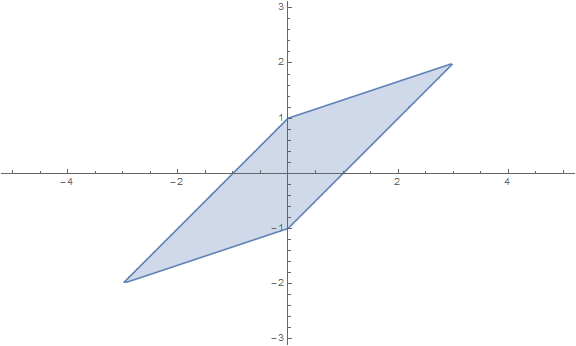
\includegraphics[width=0.7\linewidth]{Region1}\\
%\begin{align*}
%&\int\limits_{K}f(x,y)\,dxdy
%=\\=&
%\int\limits_{-\frac{5}{2}}^{\frac{5}{2}}\int\limits_{\frac{x}{3}-1}^{x+1}f(x,y)\,dydx
%+
%\int\limits_{-\frac{5}{2}}^{\frac{5}{2}}\int\limits_{x-1}^{\frac{x}{3}+1}f(x,y)\,dydx
%=\\=&
%2\int\limits_{0}^{\frac{5}{2}}\int\limits_{x-1}^{\frac{x}{3}+1}c(x+|y|)\,dydx
%\end{align*}


\subsection*{Zadanie 36}
\addcontentsline{toc}{section}{Zadanie 36}
Dwuwymiarowy wektor losowy $ (X,Y) $ ma gęstość
\begin{gather*}
f(x,y)=\left \{
\begin{array}{cll}
	0,2(x+2y) & \text{dla} & (x,y)\in[0,1] \times [0,2]   \\
	    0     & \text{dla} & (x,y)\notin[0,1]\times [0,2]
\end{array}
\right .
\qquad (x,y)\in \mathbb R ^2
\end{gather*}
Wyznaczyć:\\
$ \mathbb E \left(X|Y=y\right)\\
\mathbb E \left(X^2+1|Y=y\right) \\
\mathbb E \left(Y|X=x\right)$

Rozwiązanie:\\
\begin{minipage}[t]{0.5\linewidth}
\begin{align*}
&f_{X|Y}(x|y)
=\\=&
\frac{f(x,y)}{f_Y(y)}
=\\=&
\frac{\frac{1}{5}(x+2y)}{\int\limits_{0}^{1}\frac{1}{5}(x+2y)\,dx}
=\\=&
\frac{2(x+2y)}{4 y+1}
\end{align*}
\begin{align*}
&\mathbb E \left(X|Y=y\right)
=\\=&
\int\limits_{0}^{1}x\cdot \frac{2(x+2y)}{4 y+1}\,dx
=\\=&
\int\limits_{0}^{1}\frac{2 x^2}{4 y+1}+\frac{4 x y}{4 y+1}\,dx
=\\=&
\frac{6 y+2}{12 y+3}
\end{align*}
\end{minipage}
\begin{minipage}[t]{0.5\linewidth}
\begin{align*}
&f_{Y|X}(y|x)
=\\=&
\frac{f(x,y)}{f_X(x)}
=\\=&
\frac{\frac{1}{5}(x+2y)}{\int\limits_{0}^{2}\frac{1}{5}(x+2y)\,dy}
=\\=&
\frac{(x+2y)}{2 (x+2)}
\end{align*}
\begin{align*}
&\mathbb E \left(Y|X=x\right)
=\\=&
\int\limits_{0}^{2}y\cdot \frac{(x+2y)}{2 (x+2)}\,dy
=\\=&
\int\limits_{0}^{2}\frac{y^2}{x+2}+\frac{x y}{2 x+4}\,dy
=\\=&
\frac{3 x+8}{3 x+6}
\end{align*}
\end{minipage}\\
\begin{align*}
&\mathbb E \left(X^2+1|Y=y\right)
=\\=&
\int\limits_{0}^{1}
(x^2+1)\cdot\frac{2(x+2y)}{4 y+1}
\,dx
=\\=&
\int\limits_{0}^{1}
x^2\cdot\frac{2(x+2y)}{4 y+1}
\,dx
+
\cancelto{1}{\int\limits_{0}^{1}
\frac{2(x+2y)}{4 y+1}
\,dx}
=\\=&
\int\limits_{0}^{1}
\frac{2 x^3}{4 y+1}+\frac{4 x^2 y}{4 y+1}
\,dx
+1
=\\=&
\frac{32 y+9}{24 y+6}
\end{align*}
\chapter*{Lista 4}
\addcontentsline{toc}{chapter}{Lista 4}


\subsection*{Zadanie 37}
\addcontentsline{toc}{section}{Zadanie 37}
Niech wektor losowy $ (X,Y) $ ma gęstość daną wzorem $ \left(k\ge 2\right) $
\begin{gather*}
f_{(X,Y)}(x,y)=\left \{
\begin{array}{cll}
	k(k-1)(y-x)^{k-2} & \text{dla} & 0<x<y<1     \\
	        0         & \text{dla} & \text{else}
\end{array}
\right .
(x,y)\in \mathbb R ^2
\end{gather*}
Wyznaczyć $ \mathbb E \left(X|Y\right) $ oraz $ \mathbb E \left(Y|X\right) $. Wykorzystując otrzymane wzory obliczyć $ \mathbb E \left(X\right) $.

Rozwiązanie:\\
\begin{minipage}[t]{0.5\linewidth}
\begin{align*}
&f_{X|Y}(x|y)
=\\=&
\frac{f(x,y)}{f_Y(y)}
=\\=&
\frac{k(k-1)(y-x)^{k-2}}{\int\limits_{0}^{y}k(k-1)(y-x)^{k-2}\,dx}
=\\=&
\frac{(k-1)(y-x)^{k-2}}{y^{k-1}}
\end{align*}
\begin{align*}
&\mathbb E \left(X|Y=y\right)
=\\=&
\int\limits_{0}^{y}
x\cdot\frac{(k-1)(y-x)^{k-2}}{y^{k-1}}
\,dx
=\\=&
\int\limits_{0}^{y}
\frac{(y-x)^{k-1}}{y^{k-1}}
\,dx
=\\=&
\frac{y}{k}
\end{align*}
\end{minipage}
\begin{minipage}[t]{0.5\linewidth}
\begin{align*}
&f_{Y|X}(y|x)
=\\=&
\frac{f(x,y)}{f_X(x)}
=\\=&
\frac{k(k-1)(y-x)^{k-2}}{\int\limits_{x}^{1}k(k-1)(y-x)^{k-2}\,dy}
=\\=&
\frac{(k-1)(y-x)^{k-2}}{(1-x)^{k-1}}
\end{align*}
\begin{align*}
&\mathbb E \left(Y|X=x\right)
=\\=&
\int\limits_{x}^{1}
y\cdot \frac{(k-1)(y-x)^{k-2}}{(1-x)^{k-1}}
\,dy
=\\=&
\left .y\cdot \frac{(y-x)^{k-1}}{(1-x)^{k-1}}\right |_x^1
-
\int\limits_{x}^{1}
\frac{(y-x)^{k-1}}{(1-x)^{k-1}}
\,dy
=\\=&
1-\frac{1-x}{k}
\end{align*}
\end{minipage}\\
\begin{align*}
&E\left(X\right)
=\\=&
E\left(E\left(X|Y\right)\right)
=\\=&
\int\limits_{0}^{1}E\left(X|Y=y\right)f_Y(y)\,dy
=\\=&
\int\limits_{0}^{1}\frac{y}{k}\cdot ky^{k-1}\,dy
=\\=&
\int\limits_{0}^{1}y^k\,dy
=\\=&
\frac{1}{k+1}
\end{align*}


\subsection*{Zadanie 38}
\addcontentsline{toc}{section}{Zadanie 38}
Niech $ X_1,\dots,X_n$ będą niezależnymi zmiennymi losowymi o rozkładzie wykładniczym z parametrem $ \alpha=1 $. Znaleźć rozkład $ S_n $ oraz rozkład warunkowy $ X_1 $ pod warunkiem $ S_n $, gdzie $ S_n=\sum_{i=1}^{n}X_i $.

Rozwiązanie:
\begin{itemize}
\item $ \varphi(t)=\frac{a}{a-it} $
\item $ S_{n-1}=\sum_{i=2}^{n}X_i $
\end{itemize}
\begin{gather*}
f_{X_1,\dots,X_n}( x_1,\dots,x_n)
=
f(x_1,\dots,x_n)
=
\prod_{i=1}^{n}e^{-x_i}
=
\exp\left(-\sum_{i=1}^{n}x_i\right)
\end{gather*}
\begin{align*}
\varphi_{S_n}(t)
=
\prod_{i=1}^{n}\varphi_{x_1}(t)
=
\bigl(\varphi_{x_1}(t)\bigr)^n
=
\left(\frac{1}{1-it}\right)^n
=
\varphi_{\Gamma(n,1)}(t)
\end{align*}
\begin{align*}
f_{S_n}(t)=\frac{t^{n-1}}{(n-1)!}e^{-t}
&&
f_{S_{n-1}}(t)=\frac{t^{n-2}}{(n-2)!}e^{-t}
\end{align*}
\begin{align*}
&f_{X_1|S_n}(x|t)
=\\=&
\frac{f_{X}(x)f_{S_{n-1}}(t-x)}{f_{S_n}(t)}
=\\=&
e^{-x}\frac{(t-x)^{n-2}}{(n-2)!}e^{-(t-x)}
\frac{(n-1)!}{t^{n-1}}e^{t}
=\\=&
\frac{n-1}{t}\left(\frac{t-x}{t}\right)^{n-2}\mathbbm1_{(0,t)}(x)\cdot\mathbbm1_{(0,\infty )}(t)
\end{align*}


\subsection*{Zadanie 39}
\addcontentsline{toc}{section}{Zadanie 39}
Niech $ X_1,\dots,X_n$ będą niezależnymi zmiennymi losowymi o rozkładzie $ \mathcal N(m,1)$. Znaleźć rozkład warunkowy zmiennej warunkowe losowej $ X_1 $ pod warunkiem $ \frac{S_n}{n} $, gdzie $ S_n=\sum_{i=1}^{n}X_i $.

Rozwiązanie:
\begin{itemize}
\item $ X_1\sim \mathcal N(m,1) $
\item $ S_n\sim \mathcal N(nm,n) $
\item $ S_{n-1}=\sum_{i=2}^{n}X_i\sim \mathcal N\bigl((n-1)m,(n-1)\bigr) $
\end{itemize}
\begin{align*}
&f(X_1=x|S_n=ns)
=\\=&
\frac{f(X_1=x,S_n=ns)}{f_{S_n}(ns)}
=\\=&
\frac{f(X_1=x,S_{n-1}=ns-x)}{f_{S_n}(ns)}
=\\=&
\frac{f(X_1=x)\cdot f(S_{n-1}=ns-x)}{f_{S_n}(ns)}
=\\=&
\frac{e^{-\frac{1}{2} (x-m)^2}}{\sqrt{2 \pi }}\cdot
\frac{\exp\left(-\frac{(-m (n-1)+n s-x)^2}{2 (n-1)}\right)}{\sqrt{2 \pi }\sqrt{n-1}}\cdot
\sqrt{2 \pi } \sqrt{n} e^{\frac{(n s-m n)^2}{2 n}}
=\\=&
\frac{\sqrt{n} \exp \left(-\frac{(-m (n-1)+n s-x)^2}{2 (n-1)}+\frac{(n s-m n)^2}{2 n}-\frac{1}{2} (x-m)^2\right)}{\sqrt{2 \pi } \sqrt{n-1}}
=\\=&
\frac{e^{-\frac{n (s-x)^2}{2 (n-1)}}}{\sqrt{2 \pi } \sqrt{\frac{n-1}{n}}}
=
\frac{e^{-\frac{n (x-s)^2}{2 (n-1)}}}{\sqrt{2 \pi } \sqrt{\frac{n-1}{n}}}
\end{align*}
\begin{gather*}
\left(X_1\left |\frac{S_n}{n}\right .\right)\sim\mathcal N\left(s,\frac{n-1}{n}\right)
\end{gather*}


\subsection*{Zadanie 40 - NR}
\addcontentsline{toc}{section}{Zadanie 40 - NR}
Niech $ A_1,\dots,A_d $  będą podzbiorami otwartymi $ \mathbb R ^k $ takimi, że dla wektora losowego $ X:\Omega\to \mathbb R ^k $ mamy
\begin{gather*}
P\left\{X\in\bigcup_{i=1}^d A_i\right\}=1,\qquad
P\left\{X\in A_i\cap A_j\right\}=0,
\qquad
i\neq j
\qquad
i,j,=1,2,\dots,d
\end{gather*}
Załóżmy ponadto, ze odwzorowanie $ g:\bigcup_{i=1}^d A_i\to \mathbb R ^k $ będzie funkcją o następujących własnościach:
\begin{enumerate}[a)]
\item funkcja $ g $ jest ciągła i różnowartościowa na każdym $ A_i,\; i=1,\dots,d $
\item funkcja $ g^{-1} $ jest lokalnie lipschitzowska na każdym $ g(A_i),\;i=1\dots,d $
\end{enumerate}
Udowodnić, że jeśli $ f_X $ jest gęstością wektora losowego $ X $ to wektor losowy $ Y=g(X) $ ma gęstość postaci
\begin{gather*}
f_Y(y)=\sum_{i=1}^{d}f_X\bigl(g_i^{-1}(y)\bigr)\left|J\bigl(g_i^{-1}(y)\bigr)\right|I_{g(A_i)}(y)\qquad
y\in \mathbb R ^k
\end{gather*}

Rozwiązanie:


\subsection*{Zadanie 41}
\addcontentsline{toc}{section}{Zadanie 41}
Wektor losowy $ (X,Y) $ ma gęstość
\begin{gather*}
f(x,y)=\left \{
\begin{array}{cll}
	x+y & \text{dla} & (x,y)\in [0,1]^2 \\
	 0  & \text{dla} & (x,y)\notin [0,1]^2
\end{array}
\right .
\qquad
(x,y)\in \mathbb R ^2
\end{gather*}
\begin{enumerate}[a)]
\item Wyznaczyć gęstość $ f(U,V) $ wektora losowego $ (U,V) =  \bigl(\sin \left(\pi X\right),\cos\left (\pi Y\right)\bigr) $
\item Wyznaczyć gęstość $ f(U,V) $ wektora losowego $ (U,V)=\left(X\exp \left(\frac{Y+1}{Y}\right),Y\right) $, a następnie obliczyć $ \mathbb E \left(X\exp \left(\frac{Y+1}{Y}\right)|Y=y\right) $
\end{enumerate}
Rozwiązanie:
\begin{enumerate}[a)]
\item $ (U,V) =  \bigl(\sin \left(\pi X\right),\cos\left (\pi Y\right)\bigr) $
\begin{gather*}
(X,Y)=\left(\frac{\arcsin\left(U\right)}{\pi},
\frac{\arccos\left(V\right)}{\pi}\right)
\end{gather*}
Macierz Jakobiego\begin{gather*}
J=\left|\begin{bmatrix}
 \frac{1}{\pi  \sqrt{1-U^2}} & 0 \\
 0 & -\frac{1}{\pi  \sqrt{1-V^2}} \\
\end{bmatrix}\right|\\
\left|J\right|=\frac{1}{\pi ^2 }\cdot\frac{1}{\sqrt{1-U^2}}\cdot \frac{1}{\sqrt{1-V^2}}
\end{gather*}
Kończąc
\begin{align*}
&f_{(U,V)}(u,v)
=\\=&
f_{(X,Y)}(x,y)|J|
=\\=&
\left(\frac{\arcsin\left(U\right)}{\pi}+
\frac{\arccos\left(V\right)}{\pi}\right)\cdot
\frac{1}{\pi ^2 }\cdot\frac{1}{\sqrt{1-U^2}}\cdot \frac{1}{\sqrt{1-V^2}}\cdot
\mathbbm1_{[0,1]}(u)\cdot\mathbbm1_{[-1,1]}(v)
\end{align*}
\item $ (U,V)=\left(X\exp \left(\frac{Y+1}{Y}\right),Y\right) $
\begin{gather*}
\left \{
\begin{array}{l}
X=U e^{-\frac{V+1}{V}}\\
Y=V
\end{array}
\right .
\end{gather*}
Macierz Jakobiego
\begin{gather*}
J=\left|\begin{bmatrix}
 e^{-\frac{v+1}{v}} & \frac{ u}{v^2}e^{-\frac{v+1}{v}} \\
 0 & 1 \\
\end{bmatrix}\right|\\
|J|=e^{-\frac{v+1}{v}}
\end{gather*}
\begin{align*}
&f_{(U,V)}(u,v)
=\\=&
f_{(X,Y)}(x,y)|J|
=\\=&
\left(ue^{-\frac{v+1}{v}}+v\right)\cdot e^{-\frac{v+1}{v}}
\end{align*}
Wartość oczekiwana
\begin{align*}
f_Y(y)=\int\limits_{0}^{1}x+y\,dx
=
\frac{1}{2}+y
\end{align*}
\begin{align*}
&\mathbb E \left(X\exp \left(\frac{Y+1}{Y}\right)|Y=y\right)
=\\=&
\exp \left(\frac{y+1}{y}\right) \mathbb E \left(X|Y=y\right)
=\\=&
\exp \left(\frac{y+1}{y}\right)
\int\limits_{0}^{1}\frac{x+y}{\frac{1}{2}+y}\,dx
=\\=&
\exp \left(\frac{y+1}{y}\right)
\end{align*}
\end{enumerate}


\subsection*{Zadanie 43}
\addcontentsline{toc}{section}{Zadanie 43}
Zmienna losowa $ X $ ma rozkład jednostajny na przedziale $ (0,1) $. Wyznaczyć rozkłady zmiennych losowych $ Y=-\lambda\ln \left(1-X\right) $ i $ U=-\lambda\ln \left(X\right) $

Rozwiązanie:
\begin{gather*}
F_X(t)=t\cdot \mathbbm1_{[0,1]}(t)
\end{gather*}
\begin{minipage}[t]{0.5\linewidth}
\begin{align*}
&F_Y(t)
=\\=&
P\left(Y\le t\right)
=\\=&
P\left(-\lambda\ln \left(1-X\right)\le t\right)
=\\=&
P\left(\ln \left(1-X\right)\ge-\frac{t}{\lambda}\right)
=\\=&
P\left(1-X\ge e^{-\frac{t}{\lambda}}\right)
=\\=&
P\left(X\le 1-e^{-\frac{t}{\lambda }}\right)
=\\=&
F_X\left(1-e^{-\frac{t}{\lambda }}\right)
=\\=&
\left(1-e^{-\frac{t}{\lambda }}\right)\mathbbm1_{[0,1)}(1-e^{-\frac{t}{\lambda }})
=\\=&
\left(1-e^{-\frac{t}{\lambda }}\right)\mathbbm1_{[0,\infty )}(t)
\end{align*}
\end{minipage}
\begin{minipage}[t]{0.5\linewidth}
\begin{align*}
&F_U(t)
=\\=&
P\left(U\le t\right)
=\\=&
P\left(-\lambda\ln \left(X\right)\le t\right)
=\\=&
P\left(\ln \left(X\right)\ge -\frac{t}{\lambda}\right)
=\\=&
P\left(X\ge e^{-\frac{t}{\lambda }}\right)
=\\=&
1-F_X\left(e^{-\frac{t}{\lambda }}\right)
=\\=&
\left(1-e^{-\frac{t}{\lambda }}\right)\mathbbm1_{(0,1]}\left(e^{-\frac{t}{\lambda }}\right)
=\\=&
\left(1-e^{-\frac{t}{\lambda }}\right)\mathbbm1_{[0,\infty) }(t)
\end{align*}
\end{minipage}


\subsection*{Zadanie 44}
\addcontentsline{toc}{section}{Zadanie 44}
Zmienna losowa $ X $ ma rozkład jednostajny na przedziale $ (0,\pi) $. Wykazać, że zmienna losowa $ Y=\text{tg}(X) $ ma rozkład Cauchy'ego.

Rozwiązanie:
\begin{align*}
&F_Y(t)
=\\=&
P\left(Y\le t)\right)
=\\=&
P\left(\tg(X)\le t\right)
=\\=&
P\left(\tg(X)\le t|X\le\frac{\pi}{2}\right)
+
P\left(\tg(X)\le t|X>\frac{\pi}{2}\right)
=\\=&
P\left(X\le\arctan(t)|X\le\frac{\pi}{2}\right)\cdot P\left(X\le\frac{\pi}{2}\right)
+\\+&
P\left(X\le\arctan(t)+\pi|X>\frac{\pi}{2}\right)\cdot P\left(X>\frac{\pi}{2}\right)
=\\=&
F_{U|X\le\frac{\pi}{2}}\left(\arctan(t)\right)\cdot P\left(X\le\tfrac{\pi}{2}\right)+
F_{U|X>\frac{\pi}{2}}\left(\arctan(t)+\pi\right)\cdot P\left(X>\tfrac{\pi}{2}\right)
=\\=&
\frac{1}{\pi}\arctan(t)\cdot \frac{1}{2}+
\frac{1}{\pi}\bigl(\arctan(t)+\pi\bigr)\cdot \frac{1}{2}
=\\=&
\frac{1}{\pi}\arctan(t)+\frac{1}{2}
\end{align*}
To jest dystrybuanta rozkładu Cauchy'ego.


\subsection*{Zadanie 45}
\addcontentsline{toc}{section}{Zadanie 45}
Wykazać, że jeśli $ X $ i $ Y $ są niezależnymi zmiennymi losowymi o rozkładzie standardowym normalnym to zmienna losowa $ \frac{X}{Y} $ ma rozkład Cauchy'ego.

Rozwiązanie:
\begin{align*}
Y&=V\\
\tfrac{X}{Y}&=U\\
X&=UV
\end{align*}
\begin{gather*}
g(x,y)=(\tfrac{x}{y},y)=(u,v)\\
g^{-1}(u,v)=(uv,v)
\end{gather*}
\begin{gather*}
J=
\begin{Vmatrix}
 v & u \\
 0 & 1 \\
\end{Vmatrix}
=|v|
\end{gather*}
\begin{align*}
&f_{U,V}(u,v)
=\\=&
f_{X,Y}(uv,v)|v|
=\\=&
f_X(uv)f_Y(v)|v|
=\\=&
\frac{1}{\sqrt{2 \pi }}e^{-\frac{(uv)^2}{2}}\frac{1}{\sqrt{2 \pi }}e^{-\frac{v^2}{2}}|v|
=\\=&
\frac{|v|}{2 \pi} e^{-\frac{(uv)^2+v^2}{2}}
\end{align*}
Rozkład brzegowy
\begin{align*}
&\int\limits_{-\infty }^{\infty }
\frac{|v|}{2 \pi}e^{-\frac{(uv)^2+v^2}{2}}\,dv
=\\=&
\int\limits_{-\infty }^{\infty }
\frac{|v|}{2 \pi}e^{-\frac{ v^2\left(u^2+1\right) }{2}}\,dv
=\\=&
\frac{1}{\pi}\int\limits_{0}^{\infty }
 ve^{-\frac{ v^2\left(u^2+1\right) }{2}}\,dv
=\\=&
 \frac{1}{\pi(u^2+1)}\int\limits_{0}^{\infty }
v(u^2+1)e^{-\frac{ v^2\left(u^2+1\right) }{2}}\,dv
=\\=&
\frac{1}{\pi(u^2+1)} \int\limits_{0}^{\infty }e^{-w}\,dw
=\\=&
\frac{1}{\pi(u^2+1)}
\end{align*}
To gęstość rozkładu Cauchy'ego.


\subsection*{Zadanie 46}
\addcontentsline{toc}{section}{Zadanie 46}
Niech $ X $ i $ Y $ będą niezależnymi zmiennymi losowymi o rozkładzie wykładniczym z parametrem $ \alpha=1 $. Oznaczmy $ U=X-Y,V=Y $. Wyznaczyć gęstość wektora losowego $ (U,V) $.

Rozwiązanie
\begin{gather*}
\begin{array}{lll}
	U=X-Y &  & X=U+V \\
	V=Y   &  & Y=V
\end{array}\\
g(x,y)=(x-y,y)\\
g^{-1}(u,v)=(u+v,v)
\end{gather*}
Jakobian
\begin{gather*}
|J|=
\begin{Vmatrix}
 1 & 1 \\
 0 & 1 \\
\end{Vmatrix}=1
\end{gather*}
gęstość
\begin{align*}
&f_{U,V}(u,v)
=\\=&
f_{X,Y}(u+v,v)\cdot 1
=\\=&
e^{-u-v}e^{-v}=
e^{-u-2v}\mathbbm1_{[0,\infty )}(v)\mathbbm1_{[-v,\infty )}(u)
\end{align*}


\subsection*{Zadanie 47}
\addcontentsline{toc}{section}{Zadanie 47}
Niech $ X $ i $ Y $ będą niezależnymi zmiennymi losowymi o rozkładzie jednostajnym na przedziale $ (0,1) $. Określmy
\begin{align*}
U=\sqrt{-2\ln(X)}\cos(2\pi Y)
&&
V=\sqrt{-2\ln(X)}\sin(2\pi Y)
\end{align*}
Wykazać, że $ U $ i $ V $ są niezależnymi zmiennymi losowymi o rozkładzie normalnym $ \mathcal N(0,1) $.

Rozwiązanie:\\
Niech $ U,V\sim \mathcal N(0,1) $ oraz $ U\Perp V $
\begin{gather*}
g(x,y)=\left(\sqrt{-2\ln(x)}\cos(2\pi y),\sqrt{-2\ln(x)}\sin(2\pi y)\right)
\end{gather*}
\begin{gather*}
|J|=\begin{Vmatrix}
 -\frac{\cos (2 \pi  y)}{\sqrt{2} x \sqrt{-\log (x)}} & -2 \sqrt{2} \pi 
   \sqrt{-\log (x)} \sin (2 \pi  y) \\
 -\frac{\sin (2 \pi  y)}{\sqrt{2} x \sqrt{-\log (x)}} & 2 \sqrt{2} \pi 
   \sqrt{-\log (x)} \cos (2 \pi  y) \\
\end{Vmatrix}
=\\=
\left|-\frac{2 \pi  \cos ^2(2 \pi  y)}{x}-\frac{2 \pi  \sin ^2(2 \pi  y)}{x}\right|
=
\left|-\frac{2 \pi }{x}\right|=\frac{2 \pi }{x}
\end{gather*}
\begin{align*}
&f_{U,V}(u,v)
=\\=&
f_{X,Y}(u,v)|J|
=\\=&
\frac{e^{\frac{1}{2} \left(-u^2-v^2\right)}}{2 \pi }\cdot\frac{2 \pi }{x}
=\\=&
\frac{1}{x}\exp \left(\frac{1}{2} \left(2 \log (x) \sin ^2(2 \pi  y)+2 \log (x) \cos^2(2 \pi  y)\right)\right)
=\\=&
\frac{1}{x}\exp \left(\log (x)\right)
=\\=&
1
\end{align*}


\subsection*{Zadanie 48}
\addcontentsline{toc}{section}{Zadanie 48}
Niech $ X $ i $ Y $ będą niezależnymi zmiennymi losowymi o rozkładzie normalnym $ \mathcal N(0,1) $. Wyznaczyć gęstość wektora losowego $ (U,V) $, gdzie
\begin{align*}
U=\sqrt{X^2+Y^2}
&&
V=\frac{X}{Y}
\end{align*}
Czy zmienne losowe $ U $ i $ V $ są niezależne?

Rozwiązanie:
\begin{align*}
X=\frac{U V}{\sqrt{V^2+1}} && Y=\frac{U}{\sqrt{V^2+1}}
\end{align*}
alternatywnie
\begin{align*}
X=-\frac{U V}{\sqrt{V^2+1}} && Y=-\frac{U}{\sqrt{V^2+1}}
\end{align*}
Ale okazuje się, że w sumie ta alternatywa wcale nie jest do niczego potrzebna, bo wystarczy tylko dobrze i porządnie wyliczyć Jakobian, a nie filozofować o jakichś tam dziwnych przypadkach...
\begin{align*}
&g(x,y)=\left(\sqrt{x^2+y^2},\frac{x}{y}\right)\\
&g^{-1}(u,v)=\left( \frac{u v}{\sqrt{v^2+1}},\frac{u}{\sqrt{v^2+1}}\right)
\end{align*}
Jakobian
\begin{gather*}
|J|=
\begin{Vmatrix}
\frac{v}{\sqrt{v^2+1}} & \frac{u}{\sqrt{v^2+1}}-\frac{u
v^2}{\left(v^2+1\right)^{3/2}} \\
\frac{1}{\sqrt{v^2+1}} & -\frac{u v}{\left(v^2+1\right)^{3/2}}
\end{Vmatrix}
=
\begin{Vmatrix}
\frac{v}{\sqrt{v^2+1}} & \frac{u}{\left(v^2+1\right)^{3/2}} \\
\frac{1}{\sqrt{v^2+1}} & -\frac{u v}{\left(v^2+1\right)^{3/2}} \\
\end{Vmatrix}
=
\left|\frac{-uv^2-u}{\left(v^2+1\right)}\right|
=
\left|\frac{-u}{v^2+1}\right|
=\\=
\frac{|u|}{v^2+1}
\end{gather*}
\textsc{Bardzo istotna} jest tutaj wartość bezwzględna przy Jakobianie, bo bez tego, wszystko się posypie. Obliczanie końcowe
\begin{align*}
&f_{U,V}(u,v)
=\\=&
f_{X,Y}(x,y)|J|
=\\=&
\frac{1}{2 \pi }e^{\frac{1}{2} \left(-x^2-y^2\right)}|J|
=\\=&
f_{X,Y}\left(\frac{u v}{\sqrt{v^2+1}},\frac{u}{\sqrt{v^2+1}}\right)|J|
=\\=&
\frac{1}{2
\pi }e^{\frac{1}{2} \left(-\frac{u^2 v^2}{v^2+1}-\frac{u^2}{v^2+1}\right)}\cdot\frac{|u|}{v^2+1}
=\\=&
\frac{1}{2 \pi }e^{-\frac{u^2}{2}}\cdot\frac{|u|}{v^2+1}
\end{align*}
Rozkłady brzegowe:
\begin{align*}
&f_U(u)
=\\=&
\int\limits_{-\infty }^{\infty }
\frac{1}{2 \pi }e^{-\frac{u^2}{2}}\cdot\frac{|u|}{v^2+1}\,dv
=\\=&
\frac{|u|}{2 \pi }e^{-\frac{u^2}{2}}\cdot\bigl(\arctan(+\infty )-\arctan(-\infty )\bigr)
=\\=&
\frac{|u|}{2 \pi }e^{-\frac{u^2}{2}}\cdot\pi 
=\\=&
\frac{|u|}{2 }e^{-\frac{u^2}{2}}
\end{align*}
\begin{align*}
&f_V(v)
=\\=&
\int\limits_{-\infty }^{+\infty }
\frac{1}{2 \pi }e^{-\frac{u^2}{2}}\cdot\frac{|u|}{v^2+1}\,du
=\\=&
\frac{1}{v^2+1}\int\limits_{-\infty }^{+\infty }
\frac{|u|}{2 \pi }e^{-\frac{u^2}{2}}\cdot\,du
=\\=&
\frac{1}{v^2+1}
\left(\int\limits_{0}^{\infty}
\frac{u}{2 \pi }e^{-\frac{u^2}{2}}\,du
+
\int\limits_{-\infty }^{0}
\frac{-u}{2 \pi }e^{-\frac{u^2}{2}}\,du\right)
=\\=&
\frac{1}{v^2+1}
\left(\int\limits_{0}^{\infty}
\frac{u}{2 \pi }e^{-\frac{u^2}{2}}\,du
+
\int\limits_{0}^{\infty}
\frac{u}{2 \pi }e^{-\frac{u^2}{2}}\,du\right)
=\\=&
\frac{1}{v^2+1}\int\limits_{0}^{\infty}
\frac{u}{\pi }e^{-\frac{u^2}{2}}\,du
=\\=&
\frac{1}{\pi (v^2+1)}
\end{align*}
\begin{gather*}
f_U(u)f_V(v)=
\frac{|u|}{2 }e^{-\frac{u^2}{2}}\cdot
\frac{1}{\pi (v^2+1)}=
\frac{1}{2 \pi }e^{-\frac{u^2}{2}}\cdot\frac{|u|}{v^2+1}=
f_{U,V}(u,v)
\end{gather*}
Tak. Są niezależne.
\end{document}
